\documentclass{article}
\usepackage[utf8]{inputenc}
\usepackage{indentfirst}
\usepackage{titling}
\usepackage{geometry}
\usepackage{graphicx}
\graphicspath{ {./Images/} }
\usepackage[shortlabels]{enumitem}
\usepackage{fancyhdr}
\usepackage{ulem}
\usepackage[dvipsnames]{xcolor}
\usepackage{amssymb}
\usepackage{listings}
\usepackage{color}

\definecolor{dkgreen}{rgb}{0,0.6,0}
\definecolor{gray}{rgb}{0.5,0.5,0.5}
\definecolor{mauve}{rgb}{0.58,0,0.82}

\lstset{frame=tb,
  language=Java,
  aboveskip=3mm,
  belowskip=3mm,
  showstringspaces=false,
  columns=flexible,
  basicstyle={\small\ttfamily},
  numbers=none,
  numberstyle=\tiny\color{gray},
  keywordstyle=\color{blue},
  commentstyle=\color{dkgreen},
  stringstyle=\color{mauve},
  breaklines=true,
  breakatwhitespace=true,
  tabsize=3
}

\def\ojoin{\setbox0=\hbox{$\bowtie$}%
  \rule[-.02ex]{.25em}{.4pt}\llap{\rule[\ht0]{.25em}{.4pt}}}
\def\leftouterjoin{\mathbin{\ojoin\mkern-5.8mu\bowtie}}
\def\rightouterjoin{\mathbin{\bowtie\mkern-5.8mu\ojoin}}
\def\fullouterjoin{\mathbin{\ojoin\mkern-5.8mu\bowtie\mkern-5.8mu\ojoin}}

\renewcommand\maketitlehooka{\null\mbox{}\vfill} %para centralizar verticalmente
\renewcommand\maketitlehookd{\vfill\null}
\pagestyle{fancy}
\fancyhf{}
\rfoot{\thepage}
\lfoot{ 
\includegraphics[scale=0.01]{UA.jpg} José Mendes 107188 LEI}
\geometry{
  a4paper,
  headheight=4cm,
  top=5.5cm,
  bottom=4.5cm,
  footskip=4cm
}


\title{Segurança Informática e nas Organizações - Resumos 2}
\author{José Mendes 107188}
\date{2023/2024}

\begin{document}


\begin{titlepage}
    \maketitle
    \begin{center}
        
\includegraphics[scale=0.4]{UA.png}
    \end{center}
    \thispagestyle{empty} %remove o count da pagina
\end{titlepage}

\pagebreak

\section{Criptografia Assimétrica}

\subsection{Criptografia Assimétrica (de blocos)}

\begin{flushleft}
  \textbf{Usa um par de chaves:}
  \begin{itemize}
    \item \textbf{Chave privada:} pessoal, não transmissível;
    \item \textbf{Chave pública:} disponível a todos;
  \end{itemize}

  \vspace{2mm}

  \textbf{Permite:}
  \begin{itemize}
    \item Confidencialidade sem qualquer exchange of secrets prévia;
    \item Autenticação
    \begin{itemize}
      \item De conteúdos (integridade dos dados);
      \item De origem (atenticação da source, ou assinatura digital);
    \end{itemize}
  \end{itemize}
\end{flushleft}

\subsection{Operaçõees de uma Cifra Assimétrica}

\begin{center}
  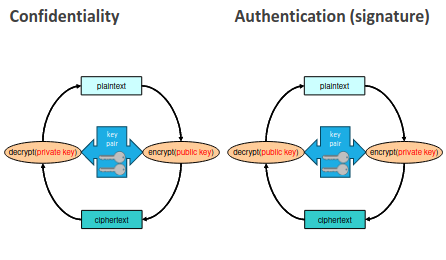
\includegraphics[scale=0.6]{1}
\end{center}

\subsection{Use Cases: Comunicação Segura}

\begin{flushleft}
  \textbf{Comunicação segura com um target (Bob)}
  \begin{itemize}
    \item A Alice encrípta o plaintext \textbf{P} com a chave pública do Bob, \textbf{Kpub\_Bob}
    \begin{itemize}
      \item \textbf{Alice: $C = \{P\}_{kpub\_bob}$}
    \end{itemize}
    \item O Bob decifra o ciphertext \textbf{C} com a sua chave privada, \textbf{Kpriv\_Bob}
    \begin{itemize}
      \item \textbf{Bob: $P' = \{C\}_{kpriv\_bob}$}
    \end{itemize}
    \item $P'$ deve ser igual a \textbf{P} (é necessário verificar)
    \item \textbf{Kpub\_Bob} precisa de ser conhecida pela Alice
  \end{itemize}
\end{flushleft}

\pagebreak

\begin{center}
  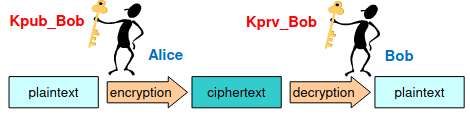
\includegraphics[scale=0.6]{2}
\end{center}

\subsection{Cifras Assimétricas}

\begin{flushleft}
  \textbf{Vantagens:}
  \begin{itemize}
    \item São um mecânismo de autenticação fundamental;
    \item Permitem explorar caracteristicas que não são possíveis com cifras simétricas;
  \end{itemize}

  \vspace{2mm}

  \textbf{Desvantagens:}
  \begin{itemize}
    \item Performance;
    \item Normalmente não são muito eficientes e consomem muita memória;
  \end{itemize}

  \vspace{2mm}
  \textbf{Problemas:}
  \begin{itemize}
    \item Distribuição confiável de chaves públicas;
    \item O lifetime do par de chaves é limitado;
  \end{itemize}

  \vspace{2mm}

  \textbf{Abordagens: problemas matemáticos complexos}
  \begin{itemize}
    \item Logaritmos discretos de números grandes;
    \item Factorização inteira de números grandes;
  \end{itemize}

  \vspace{2mm}
  \textbf{Algoritmos mais comuns:}
  \begin{itemize}
    \item RSA;
    \item ElGamal;
    \item Eliptic Curves (ECC);
  \end{itemize}

  \vspace{2mm}

  \textbf{Outras tecnicas com pares assimétricos de chaves:}
  \begin{itemize}
    \item Diffie-Hellman (key agreement);
  \end{itemize}
\end{flushleft}

\pagebreak

\subsection{RSA (Rivest, Shamir, Adelman, 1978)}

\begin{flushleft}
  \textbf{Chaves:}
  \begin{itemize}
    \item \textbf{Privada:} (d, n)
    \item \textbf{Pública:} (e, n)
  \end{itemize}

  \vspace{2mm}

  \textbf{Encriptação da chave pública (confidencialidade)}
  \begin{itemize}
    \item $C = P^e \hspace{2mm} mod \hspace{2mm} n$
    \item $P = C^d \hspace{2mm} mod \hspace{2mm} n$
  \end{itemize}

  \vspace{2mm}

  \textbf{Encriptação da chave privada (assinatura)}
  \begin{itemize}
    \item $C = P^d \hspace{2mm} mod \hspace{2mm} n$
    \item $P = C^e \hspace{2mm} mod \hspace{2mm} n$
  \end{itemize}

  \begin{center}
    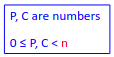
\includegraphics[scale=0.6]{3}
  \end{center}

  \textbf{Complexidade Computacional}
  \begin{itemize}
    \item Logaritmo discreto;
    \item Factorização inteira;
  \end{itemize}

  \vspace{2mm}

  \textbf{Seleção de Chaves}
  \begin{itemize}
    \item \textbf{n} grande (centenas ou milhares de bits);
    \item \textbf{$n = p \times q$} com \textbf{p} e \textbf{q} sendo números primos grandes (secretos);
    \item Escolher um \textbf{e} co-primo de \textbf{$(p-1) \times (q-1)$};
    \item Computar \textbf{d} tal que \textbf{$e \times d \equiv 1 \hspace{2mm} (mod \hspace{2mm} (p-1) \times (q-1))$};
    \item Discartar \textbf{p} e \textbf{q};
    \item O valor de \textbf{d} não pode ser facilmente computado a partir de \textbf{e} e \textbf{n} (apenas de \textbf{p} e \textbf{q});
  \end{itemize}
\end{flushleft}

\pagebreak

\subsubsection{RSA - Exemplo}

\begin{center}
  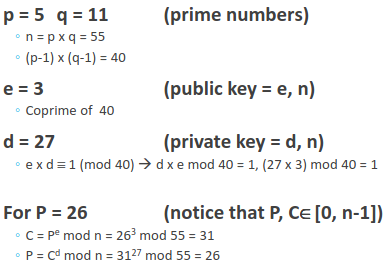
\includegraphics[scale=0.6]{4}
\end{center}

\subsection{Encriptação Hibrida}

\begin{flushleft}
  \textbf{Mistura criptografia simétrica com assimétrica}
  \begin{itemize}
    \item Usa o melhor dos dois mundos, evitando os problemas;
    \item Cifra assimétrica: usa chaves públicas (mas é lenta);
    \item Cifra simétrica: Rápida (mas com métodos fracos de troca de chaves);
  \end{itemize}

  \vspace{2mm}

  \textbf{Método}
  \begin{itemize}
    \item Obtém \textbf{$K_{pub}$} do destinatário;
    \item Gera uma chave simétrica aleatória \textbf{$K_{sym}$};
    \item Calcula \textbf{$C1 = E_{sym}(K_{sym}, P)$};
    \item Calcula \textbf{$C2 = E_{asym}(K_{pub}, K_{sym})$};
    \item Envia \textbf{$C1 + C2$};
    \begin{itemize}
      \item $C1$ é o texto encriptado com a chave simétrica;
      \item $C2$ é a chave simétrica encriptada com a chave pública do destinatário (pode também conter um IV);
    \end{itemize}
  \end{itemize}
\end{flushleft}

\subsection{Randomização de encriptações assimétricas}

\begin{flushleft}
  \textbf{Resultado de encriptações assimétricas não deterministico (não é prevísivel)}
  \begin{itemize}
    \item \textbf{N} encriptações do mesmo valor, com a mesma chave, deve produzir \textbf{N} resultados diferentes;
    \item \textbf{Objetivo:} Previnir a descoberta de valores encriptados através de tentativa e erro;
  \end{itemize}

  \vspace{2mm}

  \textbf{Abordagens:} Concatenação de um valor a encriptar com dois valores,
  um fixo (para controlo de integridade) e outro aleatório (para randomização);
\end{flushleft}

\subsubsection{OAEP (Optimal Asymmetric Encryption Padding)}

\begin{center}
  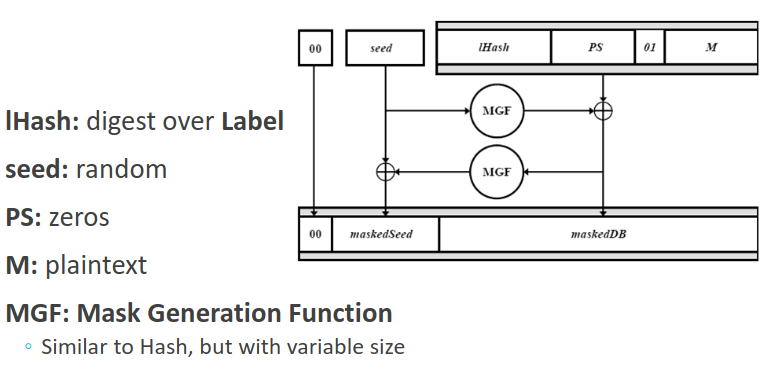
\includegraphics[scale=0.4]{5}
\end{center}

\subsection{Diffie-Hellman Key Agreement (1976)}

\begin{center}
  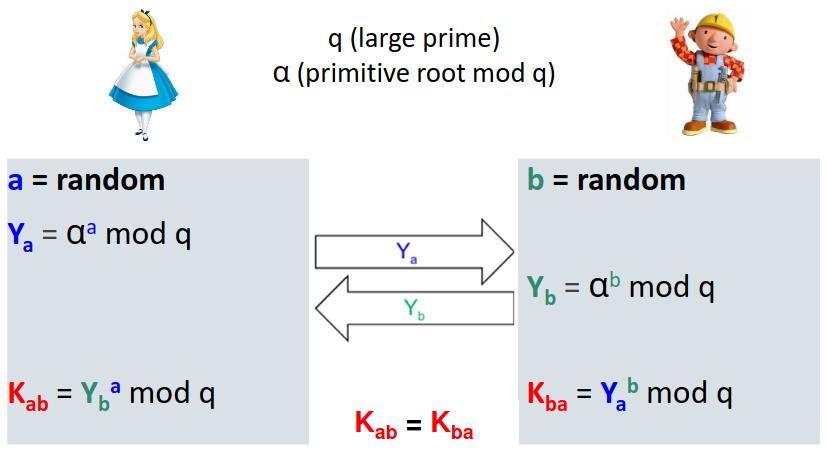
\includegraphics[scale=0.3]{6}
\end{center}

\subsubsection{DH Key Agreement: MitM Attack}

\begin{center}
  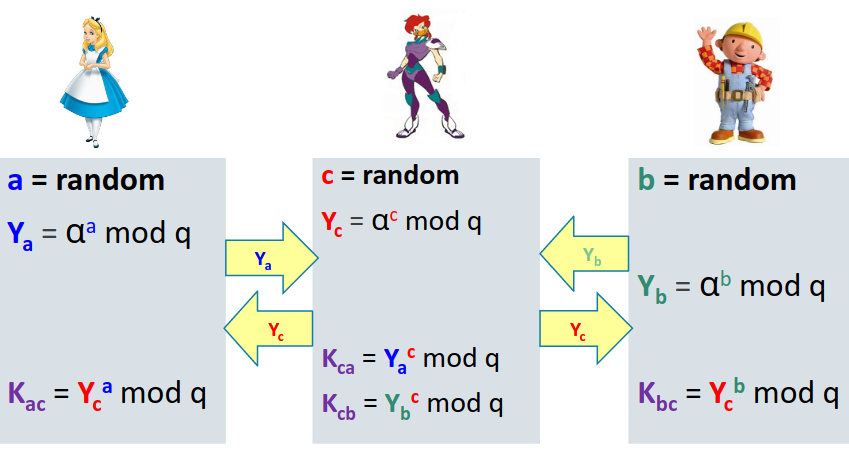
\includegraphics[scale=0.3]{7}
\end{center}

\pagebreak

\subsection{Eliptic Curve Cryptography (ECC)}

\begin{flushleft}
  \textbf{Curvas elipticas são funções específicas}
  \begin{itemize}
    \item Têm um gerador \textbf{G};
    \item Uma chave privada $K_{priv}$, é um inteiro com um máximo de
    bits permitidos pela curva;
    \item Uma chave pública $K_{pub}$, é um ponto $(x, y) = K_{priv} \times G$
    \item Dada $K_{pub}$, deve ser computacionalmente dificil determinar $K_{priv}$;
  \end{itemize}

  \begin{center}
    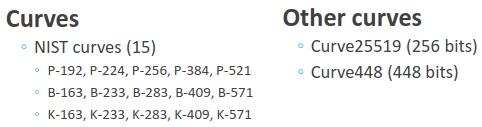
\includegraphics[scale=0.5]{9}
  \end{center}
\end{flushleft}

\subsection{ECDH: DH com ECC}

\begin{center}
  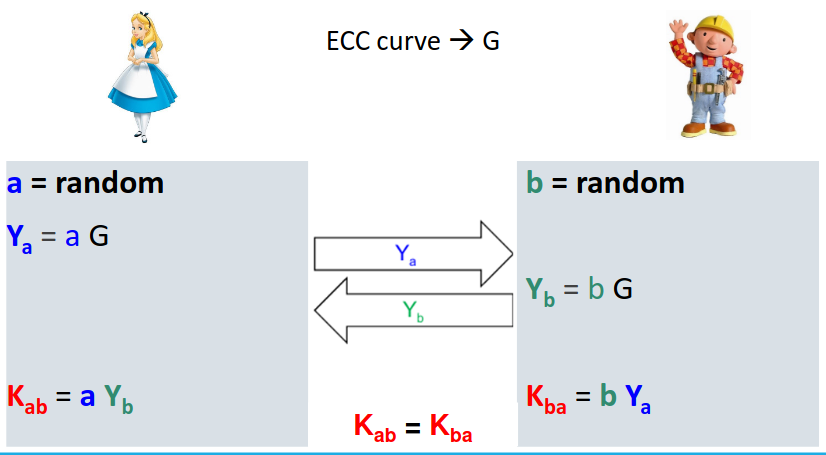
\includegraphics[scale=0.4]{8}
\end{center}

\subsection{Encriptação de chave pública com ECC}

\begin{flushleft}
  \textbf{Mistura encriptação hibrida com EDHC}

  \pagebreak

  \textbf{Método}
  \begin{itemize}
    \item Obtém $K_{pub\_recv}$ do destinatário;
    \item Gera um random $K_{priv\_send}$ com um correspondente $K_{pub\_send}$;
    \item Calcula $K_{sym} = K_{priv\_send} \times K_{pub\_recv}$;
    \item $C = E(P, K_{sym})$;
    \item Envia $C + K_{pub\_send}$;
    \vspace{2mm}
    \item Destinatário calcula $K_{sym} = K_{pub\_send} \times K_{priv\_recv}$;
    \item $P = D(C, K_{sym})$;
  \end{itemize}
\end{flushleft}

\section{Assinaturas digitais}

\subsection{Cifras Assimétricas (de blocos)}

\begin{flushleft}
  \textbf{Usa pares de chaves:}
  \begin{itemize}
    \item Uma \textbf{chave privada} (pessoal, não transmissível);
    \item Uma \textbf{chave pública} (disponível a todos);
  \end{itemize}

  \vspace{2mm}

  \textbf{Permite:}
  \begin{itemize}
    \item Confidencialidade sem qualquer exchange of secrets prévia;
    \item Autenticação
    \begin{itemize}
      \item De conteúdos (integridade dos dados);
      \item De origem (atenticação da source, ou assinatura digital);
    \end{itemize}
  \end{itemize}
\end{flushleft}

\subsection{Assinaturas Digitais}

\begin{center}
  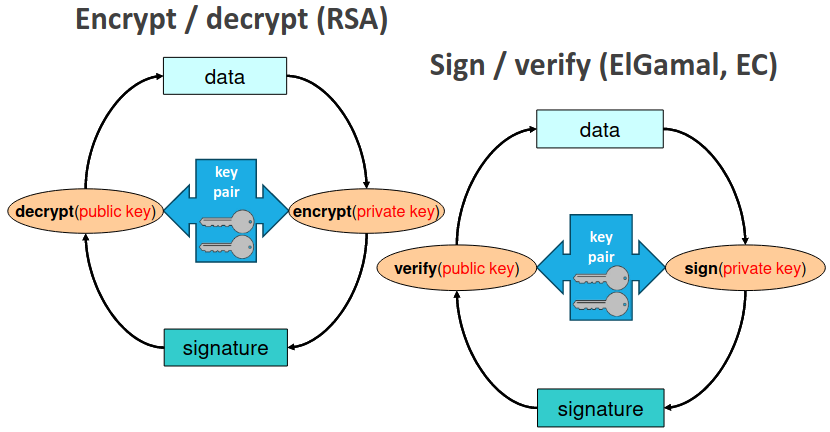
\includegraphics[scale=0.4]{10}
\end{center}

\pagebreak

\begin{flushleft}
  \textbf{Autenticação de conteúdos de um documento} - Garante a sua integridade
  (não se alterou);

  \vspace{2mm}

  \textbf{Autenticação do autor} - Garante que a identidade do criador/origem;

  \vspace{2mm}

  \textbf{Previnir repudiação de assinaturas}
  \begin{itemize}
    \item Non-repudiation (o autor não pode negar a autoria);
    \item Autores genuínos não podem negar a autoria (apenas a identidade
    do autor pode gerar uma dada assinatura);
  \end{itemize}

  \vspace{2mm}

  \textbf{Aboradgens}
  \begin{itemize}
    \item Encriptação/Decifração assimétrica ou assinatura/verificação;
    \item Funções digest (apenas para performance);
  \end{itemize}
\end{flushleft}

\begin{center}
  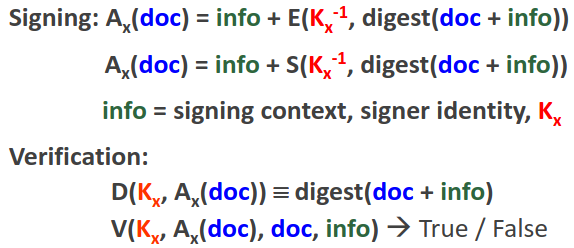
\includegraphics[scale=0.4]{11}
\end{center}

\subsubsection{Encriptação/Decifração signatures}

\begin{center}
  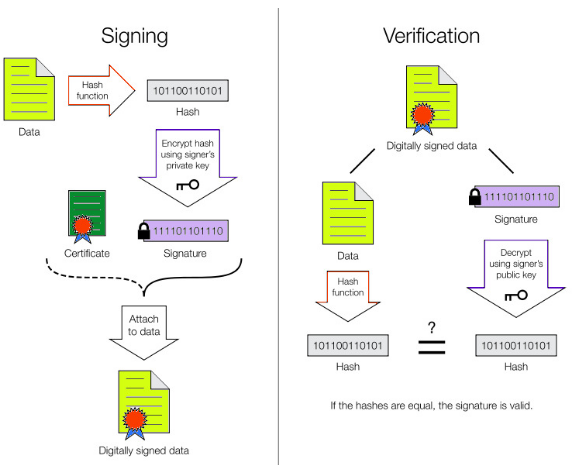
\includegraphics[scale=0.5]{12}
\end{center}

\pagebreak

\subsubsection{Assinatura digital num email: Multipart content, signature w/ certificate}

\begin{center}
  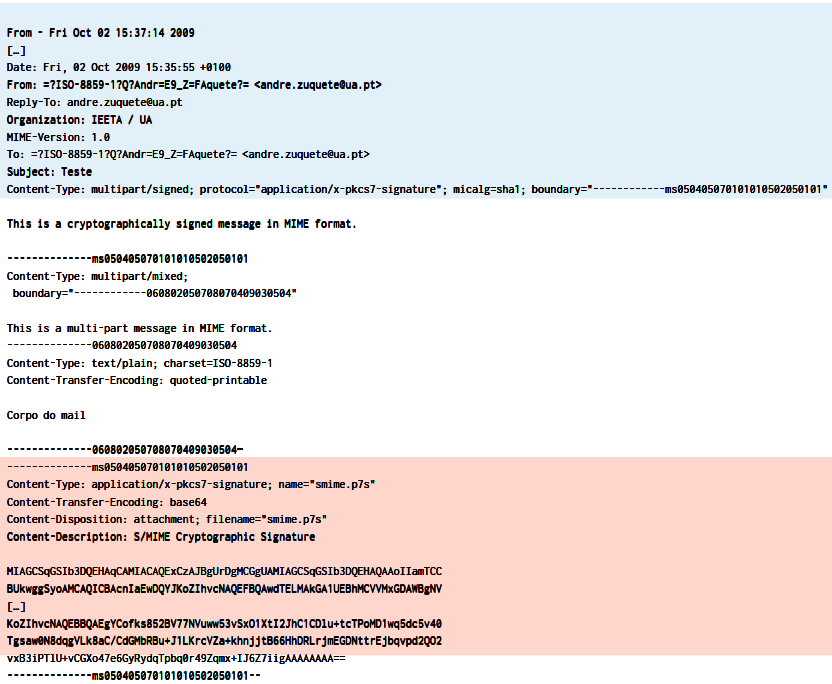
\includegraphics[scale=0.5]{13}
\end{center}

\pagebreak

\section{Derivação de chaves}

\begin{flushleft}
  \textbf{Algotitmos de cifras requerem chaves de tamanho fixo} - 56, 128, 256,\dots bits;

  \vspace{2mm}

  \textbf{Podemos derivar chaves de múltiplas origens}- shared secrets, passwords
  geradas por humanos, PIN codes e secrets de tamanho pequeno;

  \vspace{2mm}

  \textbf{Origem original pode ter baixa entropia} - reduz a dificuldade de
  ataques de força bruta, no entanto, devemos ter uma relação forte
  para uma chave útil;

  \vspace{2mm}

  \textbf{Por vezes percisamos de múltiplas chaves do mesmo material} -
  enquanto não permite encontrar o material (a password, outra chave)
  de uma chave nova;
\end{flushleft}

\subsection{Prepósitos de derivação de chaves}

\begin{flushleft}
  \textbf{Refroço de chaves: aumenta a segurança de uma password}
  \begin{itemize}
    \item Nomralmente definido por humanos;
    \item Tornando ataques de dicionário nada práticos;
  \end{itemize}

  \vspace{2mm}

  \textbf{Expansão de chaves: aumenta o tamanho de uma chave}
  \begin{itemize}
    \item Expande o tamanho que serve o algoritmo;
    \item Eventualmente deriva outras chaves relacionadas para outros algoritmos (ex: MAC);
  \end{itemize}
\end{flushleft}

\subsection{Derivação de chaves}

\begin{flushleft}
  \textbf{Derivação de chaves requer a existência de:}
  \begin{itemize}
    \item Um \textbf{salt} que trona a derivação única;
    \item Um problema difícil;
    \item Um nível de complexidade escolhido;
  \end{itemize}

  \vspace{2mm}

  \textbf{Dificuldade de Computação}
  \begin{itemize}
    \item A transformação requer recursos computacionais relevantes;
  \end{itemize}

  \vspace{2mm}

  \textbf{Dificuldade de Memória}
  \begin{itemize}
    \item A transformação requer recursos de armazenamento relevantes;
    \item Limita os ataques usando aceleração de hardware;
  \end{itemize}
\end{flushleft}

\pagebreak

\subsection{Derivação de chaves: PKBDF2}

\begin{flushleft}
  \textbf{Password Based Key Derivation Function 2}

  \vspace{2mm}

  \textbf{Produz uma chave a partir de uma password, com uma dificuldade escolhida}

  \[ K = PBKDF2(PRF, Salt, rounds, dim, password) \]

  \begin{itemize}
    \item \textbf{PRF} - Pseudo-Random-Function: função digest;
    \item \textbf{Salt} - Valor aleatório;
    \item \textbf{Rounds} - O custo computacional (dezenas ou centenas de milhares);
    \item \textbf{Dim} - Tamanho do resultado pretendido;
  \end{itemize}

  \vspace{2mm}

  \textbf{Operação: calcula operações ROUNDS x DIM a partir do PRF utilizando
  o SALT e a PASSWORD} - um tamanho maior de rounds aumenta a custo;
\end{flushleft}

\begin{center}
  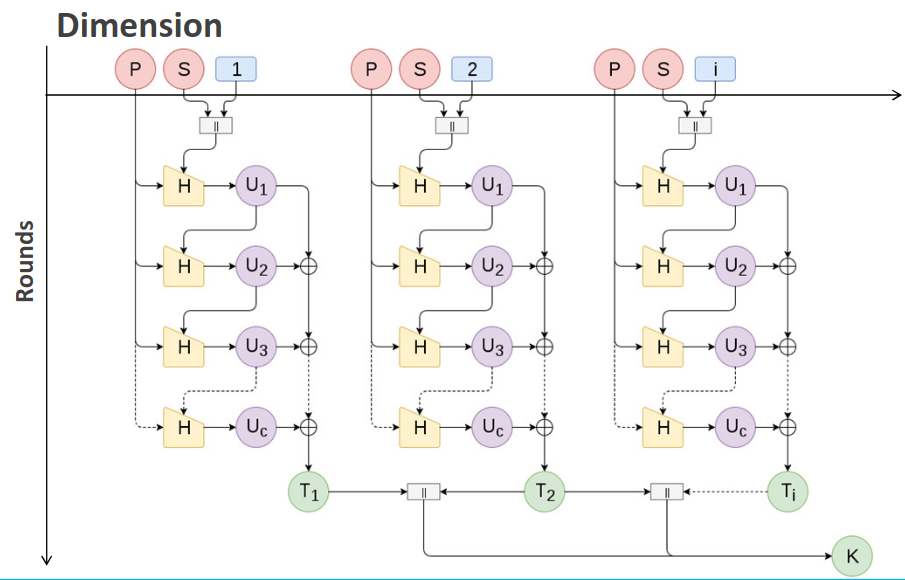
\includegraphics[scale=0.3]{14}
\end{center}

\pagebreak

\subsection{Derivação de chaves: Scrypt}

\begin{flushleft}
  \textbf{Produz uma chave com um custo de armazenamento escolhido}

  \vspace{2mm}

  \[ K = scrypt(password, salt, n, p, dim, r, hLen, Mflen) \]

  \begin{itemize}
    \item \textbf{Password} - Um segredo;
    \item \textbf{Salt} - Valor aleatório;
    \item \textbf{n} - Parâmetro de custo;
    \item \textbf{p} - Parâmetro de paralelismo $p \le (2^{32} -1) \times hLen / Mflen$;
    \item \textbf{dim} - Tamanho do resultado pretendido;
    \item \textbf{r} - Tamanho do bloco a usar (default: 8);
    \item \textbf{hLen} - Tamanho do da função digest (32 para SHA256);
    \item \textbf{Mflen} - Bytes na internal mix (default: $8 \times r$);
  \end{itemize}
\end{flushleft}

\begin{center}
  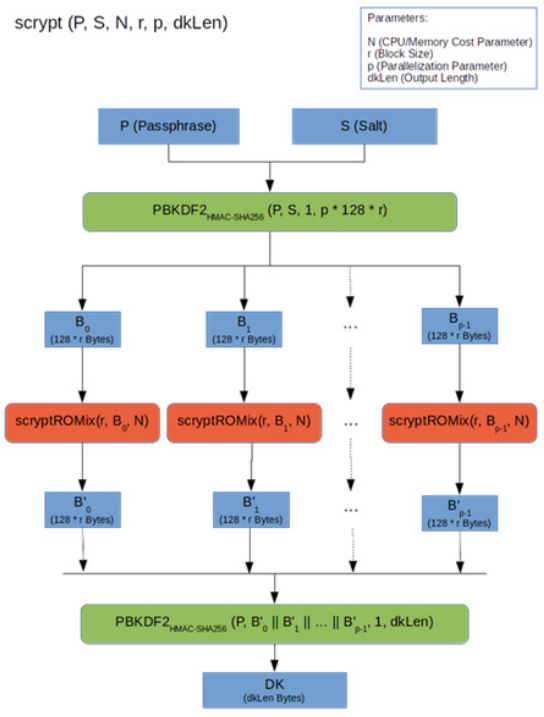
\includegraphics[scale=0.3]{15}
\end{center}

\pagebreak

\section{Gestão de chaves assimétricas}

\subsection{Problemas a resolver}

\begin{flushleft}
  \textbf{Garante um uso correto do par de chaves assimétricas}

  \begin{itemize}
     
  

    \item \textbf{Privacidade das chaves privadas}
    \begin{itemize}
      \item Garante a autenticidade;
      \item Previne a repudiação de assinaturas digitais;
    \end{itemize}

    \item \textbf{Distribuição correta de chaves públicas}
    \begin{itemize}
      \item Garante confidencialidade;
      \item Garante a correta validação de assinaturas digitais;
    \end{itemize}

  \end{itemize}

  \vspace{2mm}

  \textbf{Evolução temporal da entidade $\longleftrightarrow$ mapeamento de pares chave}

  \begin{itemize}
  
    \item \textbf{Para combater ocurrência catastróficas} (ex: perda de chaves privadas)

    \item \textbf{Para combater os requisitos de exploitations normais}
    (ex: refresh do par de chaves para reduzir riscos personificação)

  \end{itemize}

  \vspace{2mm}

  \textbf{Garante a correta geração de pares de chaves}
  \begin{itemize}
    \item \textbf{Geração aleatória de valores secretos}, de forma a poderem ser facilmente previstos;
    \item \textbf{Aumentar a eficiência sem reduzir a segurança}
    \begin{itemize}
      \item Tornar mecânismos de segurança mais eficientes;
      \item Aumentar a performance;
    \end{itemize}
  \end{itemize}
\end{flushleft}

\subsection{Objetivos}

\end{document}